%%%%%%%%%%%%%%%%%%%%%%%%%%%%%%%%%%%%%%%%%%%%%%%%%%%%%%%%%%%%%%%%%%%%%%%%%%%%%%%%
%%%%%%%%%%%%%%%%%%%%%%%%%%%%%%%%%%%%%%%%%%%%%%%%%%%%%%%%%%%%%%%%%%%%%%%%%%%%%%%%
%%% Template for AIMS Rwanda Assignments         %%%              %%%
%%% Author:   AIMS Rwanda tutors                             %%%   ###        %%%
%%% Email: tutors2017-18@aims.ac.rw                               %%%   ###        %%%
%%% Copyright: This template was designed to be used for    %%% #######      %%%
%%% the assignments at AIMS Rwanda during the academic year %%%   ###        %%%
%%% 2017-2018.                                              %%%   #########  %%%
%%% You are free to alter any part of this document for     %%%   ###   ###  %%%
%%% yourself and for distribution.                          %%%   ###   ###  %%%
%%%                                                         %%%              %%%
%%%%%%%%%%%%%%%%%%%%%%%%%%%%%%%%%%%%%%%%%%%%%%%%%%%%%%%%%%%%%%%%%%%%%%%%%%%%%%%%
%%%%%%%%%%%%%%%%%%%%%%%%%%%%%%%%%%%%%%%%%%%%%%%%%%%%%%%%%%%%%%%%%%%%%%%%%%%%%%%%


%%%%%% Ensure that you do not write the questions before each of the solutions because it is not necessary. %%%%%% 

\documentclass[12pt,a4paper]{article}

%%%%%%%%%%%%%%%%%%%%%%%%% packages %%%%%%%%%%%%%%%%%%%%%%%%
\usepackage{amsmath}
\usepackage{amssymb}
\usepackage{amsthm}
\usepackage{amsfonts}
\usepackage{graphicx}
\usepackage[all]{xy}
\usepackage{tikz}
\usepackage{verbatim}
\usepackage[left=2cm,right=2cm,top=3cm,bottom=2.5cm]{geometry}
\usepackage{hyperref}
\usepackage{caption}
\usepackage{subcaption}
\usepackage{psfrag}

%%%%%%%%%%%%%%%%%%%%% students data %%%%%%%%%%%%%%%%%%%%%%%%
\newcommand{\student}{Akor stanley}
\newcommand{\course}{ISP2}
\newcommand{\assignment}{2}

%%%%%%%%%%%%%%%%%%% using theorem style %%%%%%%%%%%%%%%%%%%%
\newtheorem{thm}{Theorem}
\newtheorem{lem}[thm]{Lemma}
\newtheorem{defn}[thm]{Definition}
\newtheorem{exa}[thm]{Example}
\newtheorem{rem}[thm]{Remark}
\newtheorem{coro}[thm]{Corollary}
\newtheorem{quest}{Question}[section]

%%%%%%%%%%%%%%  Shortcut for usual set of numbers  %%%%%%%%%%%

\newcommand{\N}{\mathbb{N}}
\newcommand{\Z}{\mathbb{Z}}
\newcommand{\Q}{\mathbb{Q}}
\newcommand{\R}{\mathbb{R}}
\newcommand{\C}{\mathbb{C}}

%%%%%%%%%%%%%%%%%%%%%%%%%%%%%%%%%%%%%%%%%%%%%%%%%%%%%%%555
\begin{document}

%%%%%%%%%%%%%%%%%%%%%%% title page %%%%%%%%%%%%%%%%%%%%%%%%%%
\thispagestyle{empty}
\begin{center}
\textbf{AFRICAN INSTITUTE FOR MATHEMATICAL SCIENCES \\[0.5cm]
(AIMS RWANDA, KIGALI)}
\vspace{1.0cm}
\end{center}

%%%%%%%%%%%%%%%%%%%%% assignment information %%%%%%%%%%%%%%%%
\noindent
\rule{17cm}{0.2cm}\\[0.3cm]
Name: \student \hfill Assignment Number: \assignment\\[0.1cm]
Course: \course \hfill Date: \today\\
\rule{17cm}{0.05cm}
\vspace{1.0cm}

\


\section*{Question 1}
\begin{itemize}
\item[(1a)]
\begin{align*}
P\left(X=x\right)&=\sum _{y=x}^{\infty} P \left(X=x/Y=y\right)P\left(Y=y\right)\\
&=\sum _{y=x}^{\infty}{y \choose x}  P^{x} \left(1-P \right) ^{y-x} \left(\frac{\lambda ^{y}e^{-\lambda}}{y!}\right)\\
&=e^{-\lambda}p^{x}\sum _{y=x}^{\infty}\frac{y!}{\left(y-x\right)!x!}\left(1-p\right)^{y-x}\frac{\lambda^{y}}{y!}\\
&=\frac{e^{-\lambda}p^{x}\lambda^{x}}{x!}\sum _{y=x}^{\infty}\frac{\left(1-p\right)^{y-x}\lambda^{y-x}}{\left(y-x\right)!}
\end{align*}

Now we have to implement a change of limit for our summation, let $q=y-x$, so that when $q=0,y=q $.
\begin{align*}
P\left(X=x\right)&=\frac{e^{-\lambda}\left(p\lambda\right)^{x}}{x!}\sum _{q=0}^{\infty}\frac{\left(\left(1-p\right)\lambda\right)^{y-x}}{\left(y-x\right)!}\\
&=\frac{e^{-\lambda}\left(p\lambda\right)^{x}}{x!}\sum _{q=0}^{\infty}\frac{\left(\left(1-p\right)\lambda\right)^{q}}{\left(q\right)!}\\
&=\frac{e^{-\lambda}\left(p\lambda\right)^{x}}{x!}e^{\left(1-p\right)\lambda}\\
&=\frac{e^{-\lambda p + \lambda-\lambda}\left(\lambda p\right)^{x}}{x!}\\
&=\frac{e^{-\lambda p}\left(\lambda p\right)^{x}}{x!}
\end{align*}
Therefore $X\backsim P\left(\lambda p\right)$.

\newpage
\item[(1b)]Here we want to show that $Y-X$ follows a poisson distribution with parameter $\lambda\left(1-p\right)$.\\
Let $Q$ be the required probability, $i.e$,\quad$Q=Y-X$, Now we are interested in finding $P\left(Q=q\right)$.
$$q=y-x$$
$$x=y-q$$
\begin{align*}
P\left(Q=q\right)&=\sum _{y=x}^{\infty} P\left(X=y-q, Y=y\right)\\
&=\sum _{y=x}^{\infty} P\left(X=y-q/ Y=y\right)P\left(Y=y\right)\\
&=\sum _{y=x}^{\infty}{y \choose y-q}  P^{y-q} \left(1-P \right) ^{y-\left(y- q\right)} \left(\frac{\lambda ^{y}e^{-\lambda}}{y!}\right)\\
&=\sum _{y=x}^{\infty} \frac{y!}{\left(y-q\right)!\left(y-\left(y-q\right)\right)!}p^{y-q} \left(1-P \right) ^{q}\left(\frac{\lambda ^{y}e^{-\lambda}}{y!}\right)\\
&=\frac{\left(1-p\right) ^{q} e^ {-\lambda}}{q!}\sum _{y=x}^{\infty}\frac{P^{y-q}\lambda ^{y-q+q}}{\left(y-q\right) !}\\
&=\frac{\left(\left(1-p\right) \lambda ^{q}\right) e^{-\lambda}}{q!}\sum _{y=x}^{\infty} \frac{\left(p \lambda\right)^{y-q}}{\left(y-q\right)!}\\
\end{align*}
From Taylor's series the summation $\sum _{q=0}^{\infty} \frac{\left(p \lambda\right)^{y-q}}{\left(y-q\right)!}=e^{p\lambda}$
\begin{align*}
&=\frac{\left(\left(1-p\right)\lambda\right)^{q} e^ {-\lambda} e^ {p \lambda}}{q!} \\
&=\frac{\left(1-p\right)\lambda^{q}}{q!} e^{-\lambda+\lambda p}\\
&=\frac{\left(1-p\right)\lambda^{q}e^{ -\lambda\left(1-p\right)}}{q!} 
\end{align*}
Therefore $Q\backsim P\left(\left(1-p\right)\lambda\right),\quad where \quad Q=Y-X$
\newpage
\item[(1c)] For $X$ and $Y-X$ to be independent their joint probability must be equal to the product of their individual probabilities.\\
\begin{align*}
P(Y-X=y-x,X=x)=P(Y-X=y-x)P(X=x)\\
\end{align*}
But:
\begin{align}
P(Y-X=y-x,X=x)&=P\left(X=x/Y-X=y-x\right)P\left(X=x \right)\\
&={y \choose x}  P^{x} \left(1-P \right) ^{y-x} \frac{e^{-\lambda p}\left(\lambda p\right)^{x}}{x!}
\end{align}
However;
\begin{align}
P\left(X=x/Y-X=y-x\right)P\left(X=x \right)&=\frac{\left(1-p\right)\lambda^{q}e^{ -\lambda\left(1-p\right)}}{q!} \frac{e^{-\lambda p}\left(\lambda p\right)^{x}}{x!}
\end{align}
where $q=y-x$, we can rewrite equation$\left(3\right)$ as;\\
\begin{align}
P\left(X=x/Y-X=y-x\right)P\left(Y-X=y-x \right)&=\frac{\left(1-p\right)\lambda^{\left( y-x\right)}e^{ -\lambda\left(1-p\right)}}{\left( y-x!\right)} \frac{e^{-\lambda p}\left(\lambda p\right)^{x}}{x!}
\end{align}
Now comparing equation$\left(2\right)$ and equation$\left(4\right)$, we can observe that they are totaly different, if the two distributions were to be independent these two equations will be the same. Hence $X$ and $Y-X$ are not independent.
\newpage
\end{itemize}
\section*{Question 2}
\begin{itemize}
\item[(1)]
.\\
\begin{figure}[h!]
\centering
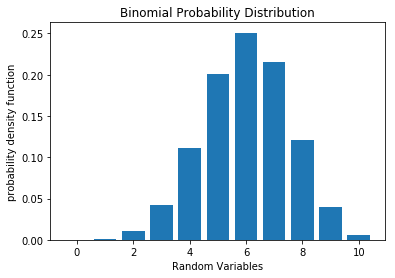
\includegraphics[scale=0.8]{Barchat.png}
\caption{Binomial Distribution}
\end{figure}
\\
The figure above shows the Binomial distribution for some random variables. 

\item[(2)]
.\\
\begin{figure}[h!]
\centering
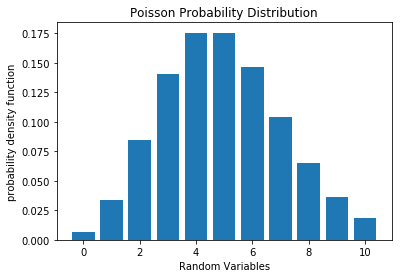
\includegraphics[scale=0.8]{Poisson.png}
\caption{Poisson Distribution}
\end{figure}
\\
The figure above shows the Poisson distribution for some random variables.
\newpage
\item[(3)]
.\\
\begin{figure}[h!]
\centering
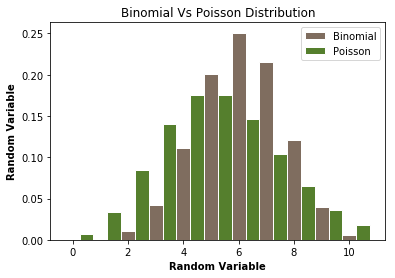
\includegraphics[scale=0.8]{BinPos.png}
\caption{Comparison between the Binomial and Poisson Distribution}
\end{figure}
\\
The figure compares the Binomial distribution with the Poisson distribution using the same random variables.
\item[(4)]
.\\
\begin{figure}[h!]
\centering
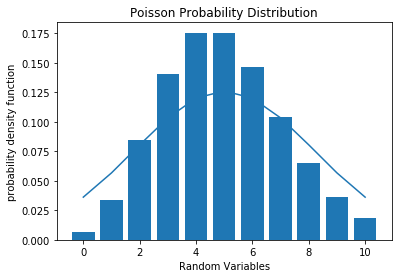
\includegraphics[scale=0.8]{NormalCurve.png}
\caption{Poisson Distribution with fitted Normal curve Distribution}
\end{figure}
\\
The figure above shows the Poisson distribution with a fitted normal curve.
\newpage
\item[(5)]
.\\
Normal distribution describes continuous information that have a symmetrical distribution, with a characteristic 'bell' form.

Binomial distribution describes the distribution of binary information from a finite sample. so it provides the chance of obtaining r events out of n trials.

Poisson distribution describes the distribution of binary information from an infinite sample. so it provides the chance of obtaining r events in a population.


\end{itemize}

\newpage
\section*{Question 3}
\begin{itemize}
\item[(1)]
\begin{itemize}
\item[(a)] $ \Gamma \left( \alpha \right) = \int\limits_0^\infty {x^{n - 1} e^{ - x} dx}$

\begin{align*}
 \Gamma \left( 1 \right) &= \int\limits_0^\infty {x^{1 - 1} e^{ - x} ds}\\
 &=\int\limits_0^\infty {x^{0} e^{ - x} dx}\\
 &=\int\limits_0^\infty {e^{ - x} dx}\\
 &=-e^{-\infty}-\left(-e^{0}\right)\\
 &=1
\end{align*}

\item[(b)]$ \Gamma \left( \frac{1}{2}\right) = \sqrt{ \Pi}$

\begin{align*}
\Gamma \left( \frac{1}{2}\right) &= \int\limits_0^\infty {x^{\frac{1}{2} - 1} e^{ - x} dx}\\
&=\int\limits_0^\infty {x^{\frac{-1}{2}} e^{ - x} dx}\\
\end{align*}

Let $u=x^{\frac{1}{2}}$, $2du=x^{\frac{-1}{2}}dx$, Substituting for $dx$ and $x^{\frac{-1}{2}}$, we shall obtain;\\

\begin{align*}
&=\int\limits_0^\infty {u} e^{ - u^{2}} \frac{2}{u} du\\
&=2\int\limits_0^\infty {} e^{ - u^{2}}du
\end{align*}
The resulting integral is a Gaussian integral which is complex to integrate, hence we have to make a change from cartesian to polar cooordinate\\

By double integration in the cartesian cordinate,its integral in the polar cordinate is a square\\

\begin{align*}
&=\left( \int\limits_0^\infty e^{-u^{2}}\right)^{2}\\
&= \int\limits_{- \infty}^\infty e^{-x^{2}}dx \int\limits_{- \infty}^\infty e^{-y^{2}}dy\\
&=\int\limits_{- \infty}^\infty \int\limits_{- \infty}^\infty e^{-\left(x^{2}+y^{2}\right)}  dxdy\\
\int \int_{R^{2}} e^{-\left(x^{2}+y^{2}\right)}dxdy
&=\int\limits_{0}^{2\Pi} \int\limits_{0}^{\infty} e^{-r^{2}}r dr d\theta\\
&=2\pi \int\limits_{0}^{\infty} re^{-r^{2}}dr\\
&=2\pi\int\limits_{- \infty}^{0} \frac{1}{2} e^{t} dt \quad \quad let \quad t=-r^{2}\\
&=\pi\int\limits_{- \infty}^{0} e^{t}dt\\
&=\pi \left(e^{0}-e^{-\infty}\right)\\
&=\pi
\end{align*}
From our previous proposition;\\
\begin{align*}
\left( \int\limits_0^\infty e^{-u^{2}}\right)^{2}&=\pi\\
\int\limits_{0}^\infty e^{-u^{2}}&=\sqrt{\pi}
\end{align*}


\item[(c)] Given  $ \Gamma \left( \alpha + 1 \right)= \alpha \Gamma \left( \alpha \right)$\\
When $\alpha$ is an integer,\quad $ \Gamma \left( \alpha + 1 \right)= \alpha ! $ , we can prove that this is true by induction.

We know that $ \Gamma \left(1\right)=1$
\\ Assume it is true for some positive integer $n$ that is $ \Gamma \left(1+n\right)=n!$\\
By our given propositon which states that $ \Gamma \left( \alpha + 1 \right)= \alpha \Gamma \left( \alpha \right)$, we want to show that it is also true for some positive integer $\left(n+1\right)$;\\
\begin{align*}
\Gamma \left( n + 2 \right) &= \Gamma \left( \left( n + 1 \right) 1 \right)\\
&=\left(n+1\right)\Gamma \left(n+ 1 \right)\\
&=\left(n+ 1 \right)\times n!\\
&=\left(n+ 1 \right)!
\end{align*}
This proves that $ \Gamma \left( \alpha + 1 \right)= \alpha \Gamma \left( \alpha \right)$.
\item[(d)] $ \int\limits_0^\infty {x^{\alpha - 1} e^{ -\beta x} dx}=$

\begin{align*}
&= \int\limits_0^\infty {x^{\alpha - 1} e^{ -\beta x}dx}
\end{align*}

Let $u=\beta x$, $du=\beta dx$ and $x=\frac{u}{\beta}$, substtituting these values into our integral above we shall obtain;

\begin{align*}
&= \int\limits_0^\infty {\left(\frac{u}{\beta}\right)^{\alpha-1} e^{ -u} \frac{du}{\beta}}
\end{align*}

Now taking the variables which are independent of $u$ out of the integral sign we shall obtain;


\begin{align*}
&=\frac{1}{\beta^{\alpha}}\int\limits_0^\infty {u^{\alpha-1} e^{ -u}du}\\
\end{align*}
 $ \Gamma \left( \alpha \right) = \int\limits_0^\infty {u^{\alpha - 1} e^{ -u} du}$ , by direct substitution, we shall obtain; \\
\begin{align*}
&=\frac{1}{\beta^{\alpha}}\times \Gamma \left( \alpha\right)\\
&=\frac{\Gamma \left( \alpha\right)}{\beta^{\alpha}}
\end{align*}

\end{itemize}
\newpage
\item[(2a)] $f\left(y\right)=\frac{\beta^{\alpha}}{\Gamma \left(\alpha \right)} y^{-\left(\alpha+1\right)}e^{-\left(\frac{\beta}{y}\right)}$\\
For $f\left(y\right)$ to be a density, the following conditions have to be satisfied;\\
\begin{itemize}
\item[1.] $f\left(y\right)\geq0$\\This condition is sufficiently satisfied because given $y \in R^{+} $, the result of the exponential will always be greater than zero.

\item[2.] $\int\limits_{0}^{\infty} f\left(y\right) dy=1$

\begin{align*}
\int\limits_0^\infty f_{y}dy&=\int\limits_{0}^{\infty}\frac{\beta^{\alpha}}{\Gamma \left(\alpha \right)} y^{-\left(\alpha+1\right)}e^{\frac{-\beta}{y}}dy\\
\end{align*}
Let $u=\frac{\beta}{y}$, $y=\frac{\beta}{u}$, $\frac{dz}{dy}=\frac{-\beta}{y^{2}}$, $dy=\frac{-\beta}{z^{2}}du$, substituting these values into the integral, we shall obtain;\\

\begin{align*}
&=\frac{\beta ^{\alpha}}{\Gamma \left(\alpha\right)}\int\limits_0^\infty \frac{u^{\alpha +1}}{\beta ^{\alpha+1}} \frac{-\beta}{u^{2}}e^{-u}du\\
&=\frac{\beta ^{\alpha}}{\Gamma \left(\alpha\right)} \frac{\beta^{-\alpha}}{1}\int\limits_0^\infty-u^{\alpha -1} e^{-u}du
\end{align*}
When we swop the limits of the integral, the negative sign of the integral changes to a positive;

\begin{align*}
&=\frac{\beta ^{\alpha}}{\Gamma \left(\alpha\right)} \frac{\beta^{-\alpha}}{1}\int\limits_\infty^0 u^{\alpha -1} e^{-u}du\\
&=\frac{\beta^{\alpha-\alpha}}{\Gamma \left(\alpha\right)}\int\limits_\infty^0 u^{\alpha -1} e^{-u}du
\end{align*}
We know that what is left of the integral is actually the gamma function.\\
\begin{align*}
&=\frac{\beta^{\alpha-\alpha}}{\Gamma \left(\alpha\right)} \Gamma \left(\alpha\right)\\
&=\frac{\Gamma \left(\alpha\right)}{\Gamma \left(\alpha\right)}\\
&=1
\end{align*}
\end{itemize}
Having satisfied these two conditions, we can can say that $f\left(y\right)$ is a density.
\newpage
\item[(3b)] Given that  
$f\left(y\right)=\frac{\beta^{\alpha}}{\Gamma \left(\alpha \right)} y^{-\left(\alpha+1\right)}e^{-\left(\frac{\beta}{y}\right)}$\\ 
\\
The expectation $E\left(y\right)$ and variance of $var\left(y\right)$ can be computed as follows;
\begin{align*}
E\left(y^{n}\right)&=\int\limits_{0}^{\infty}y^{n}\frac{\beta^{\alpha}}{\Gamma \left(\alpha \right)} y^{-\left(\alpha+1\right)}e^{-\left(\frac{\beta}{y}\right)}\\
&=\frac{\beta^\alpha}{\Gamma(\alpha)} \int_{0}^{\infty} y^{n-\alpha-1} e^{-\left(\frac{\beta}{y}\right)}dy\\ 
&=\frac{\beta^\alpha \Gamma(\alpha -n) }{\Gamma(\alpha)\beta^{\alpha - n}}\\
&= \frac{\beta^n \Gamma(\alpha -n) }{(\alpha -1) \cdots (\alpha - n) \Gamma(\alpha -n)}\\
&= \frac{\beta^n }{(\alpha -1)(\alpha -2)(\alpha -3) \cdots (\alpha - n)}
\end{align*}
Considering the case of $n=1$, all we have to do is to substitute 1 for $n$ in the equation, this gives us the expectation value.\\$$E\left(y\right)=\frac{\beta}{\left(\alpha-1\right)}$$.
\begin{align*}
var\left(y\right)&=E\left(y^{2}\right)-\left( E\left(y\right)\right)^{2}\\
&=\frac{\beta^{2}}{\left(\alpha-1\right)\cdot\left(\alpha-2\right)}-\left(\frac{\beta}{\left(\alpha-1\right)}\right)^{2}\\
&=\frac{\left(\alpha-1\right)\beta^{2}-\left(\alpha-2\right)\beta^{2}}{\left(\alpha-1\right)^{2}\left(\alpha-2\right)}\\
&=\frac{\beta^{2}}{\left(\alpha-1\right)^{2}\left(\alpha-2\right)}
\end{align*}
\newpage
\item[(2c)]$f_Y = \frac{\beta^\alpha}{\Gamma(\alpha)} \frac{1}{y^{\alpha + 1}} e^{\frac{-\beta}{y}} \quad \quad \quad\quad\quad \alpha,\beta>0$

By transformation, let $X=g\left(Y\right)=\frac{1}{Y} $, correspond to a transformation from $X$ to $Y$, $Y=\frac{1}{X}$, $\frac{dy}{dx}=  \frac{-1}{X^{2}}$\\

The tranformation of Y to X is obtained from its jacobian as follows;\\
\begin{align*}
f_X(x)&= f_Y(g^{-1}(x))|\frac{dy}{dx}| \quad\\
&=\frac{\beta^\alpha}{\Gamma(\alpha)} \frac{1}{y^{\alpha + 1}} e^{-\beta x}|\frac{dy}{dx}|\\
&=\frac{\beta^\alpha}{\Gamma(\alpha)} \frac{1}{\left(\frac{1}{x}\right)^{\alpha + 1}} e^{{-\beta x}}|\frac{-1}{x^{2}}|\\
&=\frac{\beta^\alpha}{\Gamma(\alpha)}x^{\alpha-1}e^{-\beta x}
\end{align*}

Therefore, $f_X(x)=\frac{\beta^\alpha}{\Gamma(\alpha)}x^{\alpha-1}e^{-\beta x}$,\quad is the desired result when $x,  \alpha>0$.
\item[(2d)] Taking a similar approach as in (2c), The distribution for aY, $a>0$, let $X=g(y)=aY$ and $Y=g^{-1}(X) = \frac{X}{a}$.
\begin{align*}
f_X(x) &= f_Y(g^{-1}(x))|\frac{dy}{dx}|\\
&= \frac{\beta^\alpha}{\Gamma(\alpha)} \left( \frac{a}{x}\right) ^{\alpha + 1} e^{-\frac{\beta x}{a} } \frac{1}{a}\\
&=\frac{\beta^\alpha}{\Gamma(\alpha)}\frac{a ^{\alpha + 1-1} }{x^{\alpha+1}}e^{-\frac{\beta x}{a} }\\
&=\frac{\beta^\alpha}{\Gamma(\alpha)} \frac{a^{\alpha}} {\left(x\right)^{\alpha + 1} } e^{-\frac{\beta x}{a} } \\
\end{align*}

\newpage
\item[(3a)] Given that $fx_{i}=\lambda e^{-\lambda x}\quad \quad x>0, \lambda>0$\\
The likelihood function is given by;
$$L(\lambda)=\prod _{i=1}^{n}\lambda e^{\lambda x}$$\\
By expanding the product of the geometric distibution with the p.d.f we shall obtain;
$$L(\lambda)=\lambda ^{n} e^{-\lambda \sum \limits_{i=1}^{n}xi}$$\\
Taking the log of both sides we shall obtain;
$$\ln {L(\lambda)}=n \ln{\lambda}-\lambda \sum \limits_{i=1}^{n} xi$$\\
Differentiating and equating to zero, we get;
\begin{align*}
\frac{n}{\lambda}- \sum \limits_{i=1}^{n} xi &= 0\\
\frac{n}{\lambda}&= \sum \limits_{i=1}^{n} xi\\
\lambda &=\frac{n}{\sum \limits_{i=1}^{n} xi}\\
\hat{\lambda}&=\frac{1}{\overline{x}}\\
\end{align*}
The maximum likelihood of estimator \quad$\lambda =\frac{n}{\sum \limits_{i=1}^{n} xi}=\frac{1}{\overline{x}}$
\item[(3b)] Let q=$\sum \limits_{i=1}^{n} xi$, since we know that the moment generating function of the sum of independent random variables is just the product of their moment generating function, the moment generating function of an exponential distribution is $\left(\frac{\lambda}{\lambda-t}\right)$.
\begin{align*}
Mq(t)&=\prod _{i=1}^{n}Mx_{i}(t)\\
&=\prod _{i=1}^{n}\left(\frac{\lambda}{\lambda-t}\right)\\
&=\left(\frac{\lambda}{\lambda-t}\right)^{n}
\end{align*}
Therefore the distribution of $\sum \limits_{i=1}^{n} xi\sim G\left(n,\lambda\right)$
\newpage
\item[(3c)]
	\begin{align*}
	E(\hat{\theta}) &= E\bigg(\frac{1}{n}\bigg)\\
	&= E\bigg(\frac{n}{\sum_{i=1}^{n}X_i}\bigg)\\
	=& nE\bigg(\frac{1}{y}\bigg)\\
	=& n\int_{0}^{\infty}\frac{1}{y}\frac{\lambda ^n}{\varGamma(n)}y^{n-1}e^{-\lambda y}dy\\
	\end{align*}
	Let $u=\lambda y ,du =\lambda dy ,y = \frac{u}{\lambda}$		
\begin{align*}
	E(\hat{\lambda})	=& n\frac{\lambda ^n}{\varGamma(n)}\int_{0}^{\infty}\bigg(\frac{u}{\lambda}\bigg)^{n-2}e^{-u}\frac{du}{\lambda}\\
	=& n\frac{\lambda ^n}{\varGamma(n)}\int_{0}^{\infty}\bigg(\frac{u}{\lambda}\bigg)^{n-2}e^{-u}du\\
	=&  n\frac{\lambda ^{n-1}}{\varGamma(n)}\frac{1}{\lambda^{n-1}\lambda^{-1}}{\int_{0}^{\infty}u^{n-2}e^{-u}du}\\
=&\frac{n\lambda^n}{(n-1)\varGamma(n-1)}\varGamma(n-1)\\
&= \frac{n}{n-1}\lambda
	\end{align*} 
Since $E(\hat{\theta})\neq\lambda$, $\hat{\lambda}$ is not an unbiased estimator.

\item[(3d)]
$f_{y}\left(y\right)=\frac{1}{2^{\frac{n}{2}}\Gamma\left(\frac{n}{2}\right)}y^{\frac{n}{2}-1}e^{\frac{-y}{2}}$
\end{itemize}
\end{document}
